\documentclass[xcolor={usenames,svgnames}]{beamer}

\usepackage[francais]{babel}
\usepackage{rtxslides}
\usepackage{listings}
\usepackage{tikz}
\usetikzlibrary{shapes,fit}

\definecolor{grey}{rgb}{0.10,0.10,0.10}
\definecolor{rBlue}{rgb}{0.0,0.44,0.96}
\definecolor{rRed}{rgb}{0.6,0.0,0.0}
\definecolor{rGreen}{rgb}{0.0,0.4,0.0}

\definecolor{tblR}{rgb}{1.0,0.0,0.0}
\definecolor{tblG}{rgb}{0.0,1.0,0.0}
\definecolor{tblB}{rgb}{0.3,0.7,1.0}

\lstdefinelanguage{rathaxes}%
{
	morekeywords={
        interface, extend,                      % interfaces : decl
        device, configuration, driver,          % devices
        with, values,                           % backend+interface
        builtin, provided, required, optional,  % interfaces: implem
        type, sequence, variable,               % general: element type
        use, pointcut, chunk,                   % for aspectual concepts
        template                                % backend
    },%
	sensitive=true,%
	morecomment=[l][\color{rRed}]{//},%
 	morecomment=[l][\color{rRed}]{\#},%
	morecomment=[s][\color{rRed}]{/*}{*/},%
	morestring=[b][\color{rGreen}]",%
	morestring=[b][\color{rGreen}]',%
	keywordstyle={\color{rBlue}}%
}[keywords,comments,strings]

\definecolor{lstbackground}{rgb}{0.0, 0.0, 0.0}
\definecolor{lstcomment}{rgb}{0, 0.12, 0.76}
\definecolor{lstkeyword}{rgb}{0.23, 0.13, 0.78}
\definecolor{lststring}{rgb}{0.67, 0.7, 0.13}
\definecolor{lstidentifier}{rgb}{0.82, 0.82, 0.82}

\linespread{1.0}
\lstset{
    language=rathaxes,
    tabsize=2,
    captionpos=b,
    emptylines=0,
    frame=single,
    breaklines=false,
    breakatwhitespace=false,        % sets if automatic breaks should only happen at whitespace
    extendedchars=false,
    showstringspaces=false,
    showspaces=false,
    showtabs=false,
    framexrightmargin=-100pt,
    basicstyle=\color{white}\tiny\ttfamily,
    numbers=right,                   % where to put the line-numbers
    numberstyle=\scriptsize\ttfamily,
    stepnumber=1,                   % the step between two line-numbers. If it's 1, each line
    numbersep=-90pt,                  % how far the line-numbers are from the code
    keywordstyle=\color{lstkeyword},
    commentstyle=\color{lstcomment},
    identifierstyle=\color{lstidentifier},
    stringstyle=\color{lststring},
    backgroundcolor=\color{lstbackground},
    escapeinside={\%*}{*)},         % if you want to add a comment within your code
    morekeywords={*,...}            % if you want to add more keywords to the set
}

\title{\rtx\ -- RMLL 2011}
\date{8 Juillet 2011}
\author{\rtx \\ \texttt{www.rathaxes.org} \\ L. Auroux \& D.Pineau }

\definecolor{lightred}{RGB}{147,36,33}
\tikzset{componentarrow/.style={->, >=stealth, color=rathaxesred, ultra thick}}

\newcommand{\cemph}[1]{{\itshape{\textcolor{rathaxesred}{#1}}}}

\newcommand{\tred}[1]{\textcolor{rathaxesred}{#1}}

\tikzset{warrow/.style={->, >=stealth, color=white, ultra thick}}

\tikzset{graybox/.style={draw,rectangle,rounded corners=3pt,very thick,densely dashed,color=gray!75,text=white}}
\tikzset{redbox/.style={draw,rectangle,rounded corners=5pt,ultra thick,color=rathaxesred,text=white}}
\tikzset{redcontainer/.style={draw,rectangle,rounded corners=5pt,ultra thick,color=rathaxesred,text=white,minimum height=3.5cm,minimum width=2.5cm}}

\begin{document}

\begin{frame}
\titlepage
\end{frame}

\begin{frame}{Historique du projet}
\begin{center}
	\begin{itemize}
		\item	Thèse de L.Reveillere "Devil" (2002);
		\item	Début du projet (2007) LSE - EIP Epitech;
		\item	RMLL / T-DOSE (2008).
	\end{itemize}
\end{center}
\end{frame}


\begin{frame}{Pilotes de périphériques}
\begin{center}
\only<1>{\LARGE{Souvent \cemph{\Huge{instables}} et \cemph{\Huge{bancals}}}}
\only<2> of Windows Vista \tred{crashes} caused by \tred{Nvidia drivers}~»}}}

\vspace{1cm}
\raggedleft\large{2.6.39: \itshape{\rmfamily{«~les pilotes (\tred{65 \% des patches})~»}} (patrick\_g)}

\vspace{1cm}
\large{2.6.35: \itshape{\rmfamily{«~les \tred{deux tiers des changements} dans les pilotes~»}}}
}
\end{center}
\end{frame}

\begin{frame}{Développement de pilotes de périphériques}
\begin{center}
\only<1>{\Large{Une tâche \cemph{\LARGE{difficile}}, \cemph{\LARGE{longue}} et \cemph{\LARGE{fastidieuse}}}}
\only<2>{\Large{%
\begin{itemize}
\item Compétences requises ;
\item Portabilité ;
\item Maintenance.
\end{itemize}
}}
\end{center}
\end{frame}

\begin{frame}{Objectifs du DSL \rtx}
\begin{center}
\only<1>{\Large{\cemph{\LARGE{Simplifier}} les cycles de développement}}
\only<2>{\Large{\begin{itemize}
\item Abstraction de la plateforme ;
\item Vérifications statiques ;
\item Séparation des compétences.
\end{itemize}}}
\end{center}
\end{frame}

\begin{frame}[fragile]{Qu'est ce qu'un driver}
	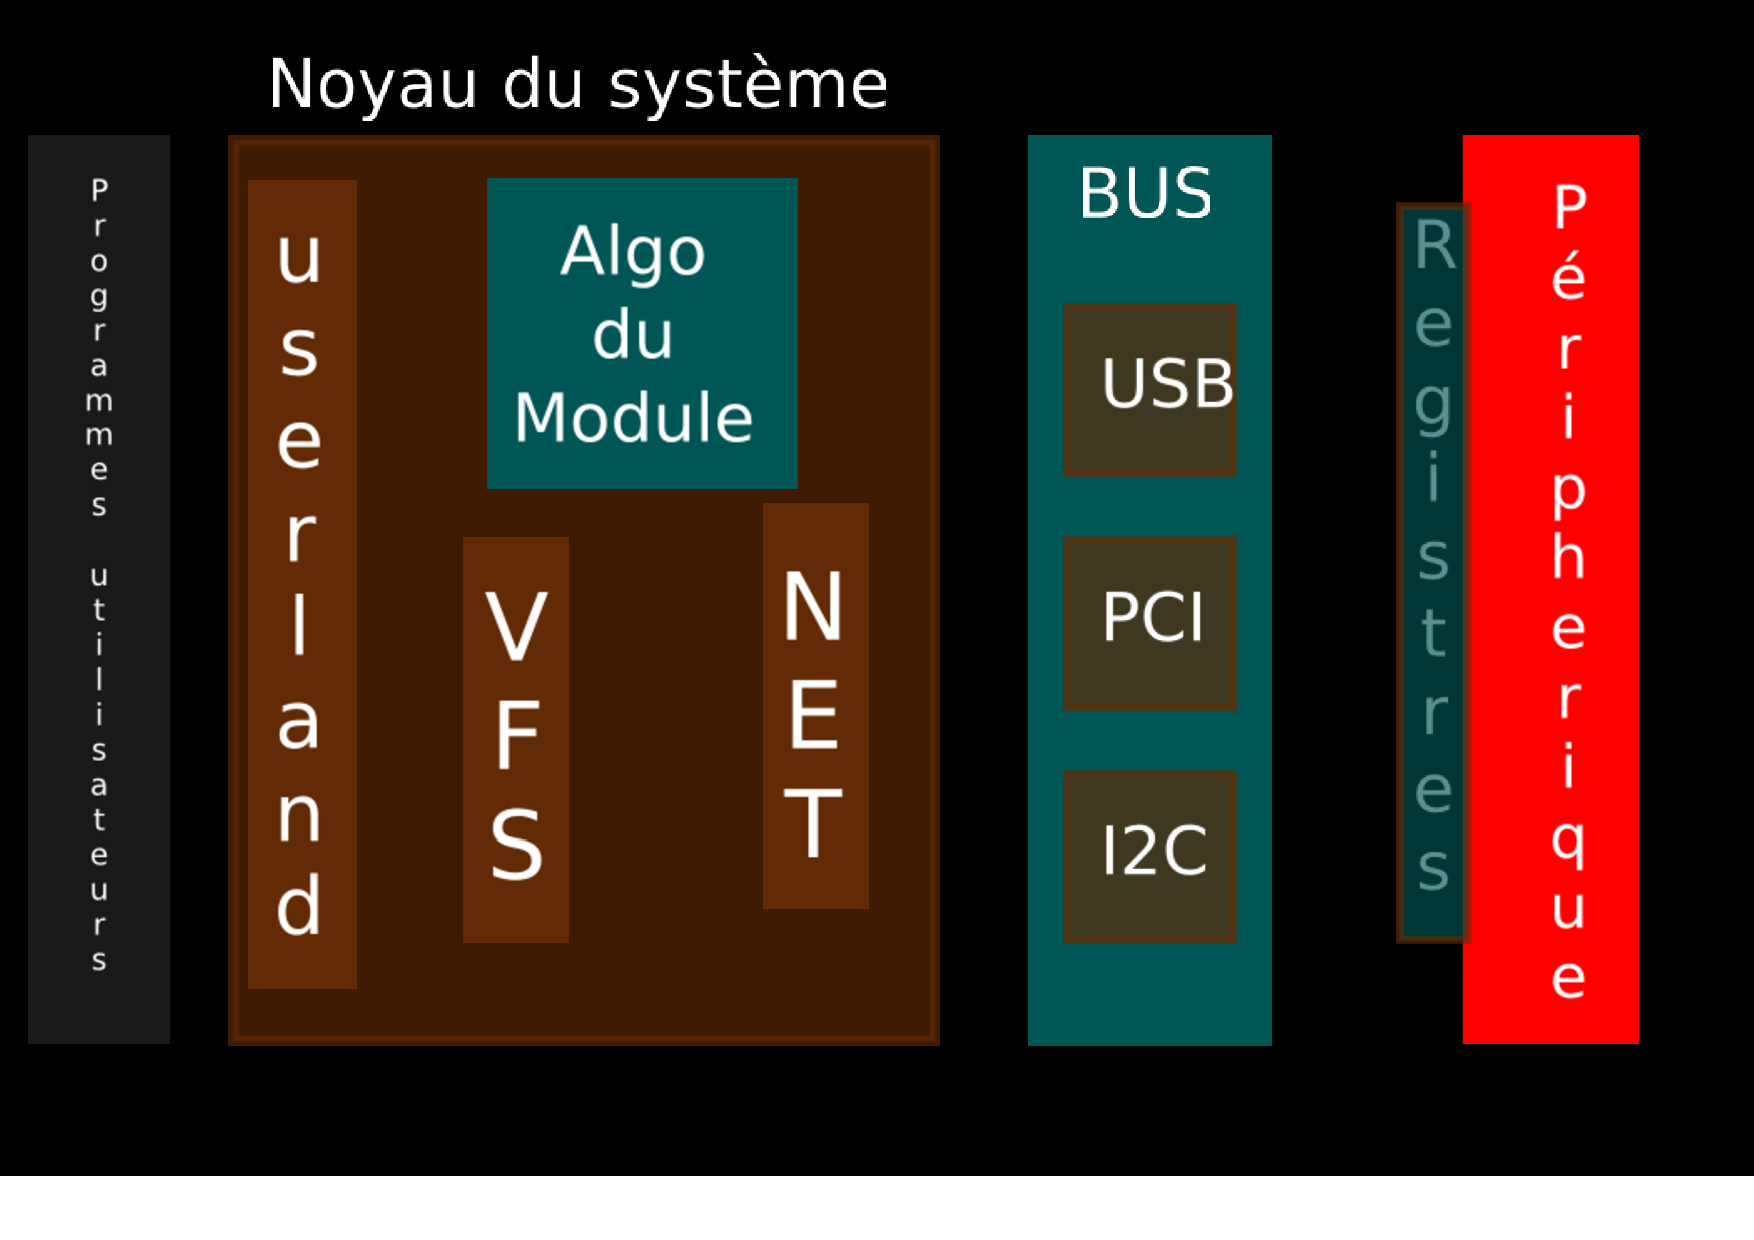
\includegraphics[scale=0.37]{stateofdevice.pdf}
\end{frame}

\begin{frame}{Outils utilisés}
	\begin{center}
	\begin{itemize}
		\item	Langage Codeworker (www.codeworker.org LGPL);
		\item	Front end C : Cnorm (code.google.com/p/cnorm LGPL);
	\end{itemize}
	\end{center}
\end{frame}

\begin{frame}{Première approche}
	\begin{center}
	\large{Démonstration}
	\end{center}
\end{frame}

\begin{frame}{Génération d'un pilote}
\only<1>{\begin{tikzpicture}[overlay]
\node (RTX) at (2,2.5) {
\includegraphics[height=1.5cm]{icons/rtx}};
\node[redbox] (COMPILER) at (2,-0.5) {Compilateur};
\node (C) at (2,-3.5) {
\includegraphics[height=1.5cm]{icons/c}};

\draw[warrow] (RTX)--(COMPILER);
\draw[warrow] (COMPILER)--(C);

\draw (RTX.north east) node[below right]{%
\begin{minipage}{9cm}
\large{Description du pilote :}
\small{
\begin{itemize}
\item Description du matériel ;
\item Algorithmes ;
\item Paramètres spécifiques à chaque système.
\end{itemize}}
\end{minipage}};

\draw (C.north east) node [below right]{\large{Module noyau}};
\end{tikzpicture}}

\only<2>{\begin{tikzpicture}[overlay]
\node (RTX) at (2,2.5) {
\includegraphics[height=1.5cm]{icons/rtx}};
\node[redbox] (COMPILER) at (2,-0.5) {Compilateur};
\node (C) at (2,-3.5) {
\includegraphics[height=1.5cm]{icons/c}};

\draw[warrow] (RTX)--(COMPILER);
\draw[warrow] (COMPILER)--(C);

\node[below right] (H1) at (RTX.north east) {%
\begin{minipage}{7.5cm}
\large{Description du pilote :} \\
\small{\texttt{
device Pipe use LKM, CharDev, Algorithms \{
\hspace*{1ex} open(Context ctx) \{ \\
\hspace*{2ex} log(“Open called on device Pipe”); \\
\hspace*{1ex} \} \\
\}
}}
\end{minipage}};
\draw (C.north east) node [below right]{\large{Module noyau}};
\end{tikzpicture}}

\only<3>{\begin{tikzpicture}[overlay]
\node[opacity=0.3] (RTX) at (2,2.5) {
\includegraphics[height=1.5cm]{icons/rtx}};
\node[redcontainer] (COMPILER) at (2,-0.5) {};
\node[opacity=0.3] (C) at (2,-3.5) {
\includegraphics[height=1.5cm]{icons/c}};

\draw[warrow,opacity=0.3] (RTX)--(COMPILER);
\draw[warrow,opacity=0.3] (COMPILER)--(C);

\draw (RTX.north east) node[below right, opacity=0.3]{\large{Description du pilote}};
\draw (COMPILER.south east) node[above right]{\Large{Compilateur}};
\draw (C.north east) node [below right, opacity=0.3]{\large{Module noyau}};
\end{tikzpicture}}

\only<4>{\begin{tikzpicture}[overlay]
\node[opacity=0.3] (RTX) at (2,2.5) {
\includegraphics[height=1.5cm]{icons/rtx}};
\draw (RTX.north east) node[below right, opacity=0.3]{\large{Description du pilote}};

\node[opacity=0.3] (C) at (2,-3.5) {
\includegraphics[height=1.5cm]{icons/c}};

\node[graybox] (AST1) at (2,0.5){\texttt{AST}};
\draw[warrow] (RTX)--(AST1);

%\node[graybox] (AST2) at (2,-1.5) {\texttt{AST}};
%\draw[warrow] (AST2)--(C);

\node[redcontainer] (COMPILER) at (2,-0.5) {};
\draw (COMPILER.south east) node[above right]{\Large{Compilateur}};

%\node[graybox] (RTXLINK) at (COMPILER.center) {\texttt{RTX\_Link}};
%\draw[warrow] (AST1)--(RTXLINK);
%\draw[warrow] (RTXLINK)--(AST2);

\draw[warrow,opacity=0.3] (COMPILER)--(C);
\draw (C.north east) node [below right, opacity=0.3]{\large{Module noyau}};
\end{tikzpicture}}

\only<5>{\begin{tikzpicture}[overlay]
\node[opacity=0.3] (RTX) at (2,2.5) {
\includegraphics[height=1.5cm]{icons/rtx}};
\draw (RTX.north east) node[below right, opacity=0.3]{\large{Description du pilote}};

\node[opacity=0.3] (C) at (2,-3.5) {
\includegraphics[height=1.5cm]{icons/c}};

\node[graybox] (AST1) at (2,0.5){\texttt{AST}};
\draw[warrow] (RTX)--(AST1);

%\node[graybox] (AST2) at (2,-1.5) {\texttt{AST}};
%\draw[warrow] (AST2)--(C);

\node[redcontainer] (COMPILER) at (2,-0.5) {};
\draw (COMPILER.south east) node[above right]{\Large{Compilateur}};

\node[graybox] (RTXLINK) at (COMPILER.center) {\texttt{RTX\_Link}};
\draw[warrow] (AST1)--(RTXLINK);
%\draw[warrow] (RTXLINK)--(AST2);

\draw[warrow,opacity=0.3] (COMPILER)--(C);
\draw (C.north east) node [below right, opacity=0.3]{\large{Module noyau}};
\end{tikzpicture}}

\only<6>{\begin{tikzpicture}[overlay]
\node[opacity=0.3] (RTX) at (2,2.5) {
\includegraphics[height=1.5cm]{icons/rtx}};
\draw (RTX.north east) node[below right, opacity=0.3]{\large{Description du pilote}};

\node[opacity=0.3] (C) at (2,-3.5) {
\includegraphics[height=1.5cm]{icons/c}};

\node[graybox] (AST1) at (2,0.5){\texttt{AST}};
\draw[warrow] (RTX)--(AST1);

%\node[graybox] (AST2) at (2,-1.5) {\texttt{AST}};
%\draw[warrow] (AST2)--(C);

\node[redcontainer] (COMPILER) at (2,-0.5) {};
\draw (COMPILER.south east) node[above right]{\Large{Compilateur}};

\node[graybox] (RTXLINK) at (COMPILER.center) {\texttt{RTX\_Link}};
\draw[warrow] (AST1)--(RTXLINK);
%\draw[warrow] (RTXLINK)--(AST2);

\draw[warrow,opacity=0.3] (COMPILER)--(C);

\node (RTI) at (4.5,0.85) {
\includegraphics[height=1.3cm]{icons/rti}};
\draw (RTI.east) node[above right]{\Large{Interfaces}};
\draw[warrow] (RTI.west)--(RTXLINK.north);
\draw (C.north east) node [below right, opacity=0.3]{\large{Module noyau}};
\end{tikzpicture}}

\only<7>{\begin{tikzpicture}[overlay]
\node[opacity=0.3] (RTX) at (2,2.5) {
\includegraphics[height=1.5cm]{icons/rtx}};
\draw (RTX.north east) node[below right, opacity=0.3]{\large{Description du pilote}};

\node[opacity=0.3] (C) at (2,-3.5) {
\includegraphics[height=1.5cm]{icons/c}};

\node[graybox] (AST1) at (2,0.5){\texttt{AST}};
\draw[warrow] (RTX)--(AST1);

%\node[graybox] (AST2) at (2,-1.5) {\texttt{AST}};
%\draw[warrow] (AST2)--(C);

\node[redcontainer] (COMPILER) at (2,-0.5) {};
\draw (COMPILER.south east) node[above right]{\Large{Compilateur}};

\node[graybox] (RTXLINK) at (COMPILER.center) {\texttt{RTX\_Link}};
\draw[warrow] (AST1)--(RTXLINK);
%\draw[warrow] (RTXLINK)--(AST2);

\draw[warrow,opacity=0.3] (COMPILER)--(C);

\node (RTI) at (4.5,0.85) {
\includegraphics[height=1.3cm]{icons/rti}};
\draw (RTI.east) node[above right]{\Large{Interfaces}};
\draw[warrow] (RTI.west)--(RTXLINK.north);

\node (BLT) at (4.5,-0.5) {
\includegraphics[height=1.3cm]{icons/blt}};
\draw (BLT.east) node[above right]{\Large{Patrons de code}};
\draw[warrow] (BLT.west)--(RTXLINK);
\draw (C.north east) node [below right, opacity=0.3]{\large{Module noyau}};
\end{tikzpicture}}

\only<8>{\begin{tikzpicture}[overlay]
\node[opacity=0.3] (RTX) at (2,2.5) {
\includegraphics[height=1.5cm]{icons/rtx}};
\draw (RTX.north east) node[below right, opacity=0.3]{\large{Description du pilote}};

\node[opacity=0.3] (C) at (2,-3.5) {
\includegraphics[height=1.5cm]{icons/c}};

\node[graybox] (AST1) at (2,0.5){\texttt{AST}};
\draw[warrow] (RTX)--(AST1);

\node[graybox] (AST2) at (2,-1.5) {\texttt{AST}};
\draw[warrow] (AST2)--(C);

\node[redcontainer] (COMPILER) at (2,-0.5) {};
\draw (COMPILER.south east) node[above right]{\Large{Compilateur}};

\node[graybox] (RTXLINK) at (COMPILER.center) {\texttt{RTX\_Link}};
\draw[warrow] (AST1)--(RTXLINK);
\draw[warrow] (RTXLINK)--(AST2);

\node (RTI) at (4.5,0.85) {
\includegraphics[height=1.3cm]{icons/rti}};
\draw (RTI.east) node[above right]{\Large{Interfaces}};
\draw[warrow] (RTI.west)--(RTXLINK.north);

\node (BLT) at (4.5,-0.5) {
\includegraphics[height=1.3cm]{icons/blt}};
\draw (BLT.east) node[above right]{\Large{Patrons de code}};
\draw[warrow] (BLT.west)--(RTXLINK);
\draw (C.north east) node [below right, opacity=0.3]{\large{Module noyau}};
\end{tikzpicture}}
\end{frame}

\begin{frame}{Interfaces et patrons de code}
\begin{tikzpicture}[overlay]
\node (RTI) at (1.2,1.6) {
\includegraphics[height=1.5cm]{icons/rti}};

\draw (RTI.north east) node[below right]{%
\begin{minipage}{10cm}
Décrivent un \emph{«~sous système~»} avec :
\begin{itemize}
\item Des types ;
\item Des séquences ;
\item Des variables de configuration.
\end{itemize}
\end{minipage}};
\end{tikzpicture}
\end{frame}

\begin{frame}[fragile]{Interfaces et patrons de code}
\begin{tikzpicture}[overlay]
\node (RTI) at (1.2,1.6) {
\includegraphics[height=1.5cm]{icons/rti}};

\draw (RTI.east) node[right]{%
\begin{minipage}{10cm}
\begin{lstlisting}
interface CharDev : LKM {
  provided type        Context;
  required sequence    open(Context) {
     use pointcut      LKM::GLOBAL_CODE_DEFINITION;
     use pointcut      LKM::INIT_LKM_FPTRS;
     provided pointcut ALGO;
  }
  required variable identifier  OS;
  required variable serial      version;
}
\end{lstlisting}
\end{minipage}};
\end{tikzpicture}
\end{frame}

\begin{frame}[fragile]{Interfaces et patrons de code}
\begin{tikzpicture}[overlay]
\node (RTI) at (1.2,1.6) {
\includegraphics[height=1.5cm]{icons/rti}};

\draw (RTI.east) node[right]{%
\begin{minipage}{10cm}
\begin{lstlisting}
interface CharDev : LKM {
  provided type        Context;
  required sequence    open(Context) {
     use pointcut      LKM::GLOBAL_CODE_DEFINITION;
     use pointcut      LKM::INIT_LKM_FPTRS;
     provided pointcut ALGO;
  }
  required variable identifier  OS;
  required variable serial      version;
}
\end{lstlisting}
\end{minipage}};

\node (BLT) at (1.2,-2.2) {
\includegraphics[height=1.5cm]{icons/blt}};

\draw (BLT.north east) node[below right]{%
\begin{minipage}{10cm}
Implémentations des interfaces pour chaque OS :
\begin{itemize}
\item Templates de types ;
\item Templates de séquences.
\end{itemize}
\end{minipage}};
\end{tikzpicture}
\end{frame}

\begin{frame}[fragile]{Interfaces et patrons de code}
\begin{tikzpicture}[overlay]
\node (RTI) at (1.2,1.6) {
\includegraphics[height=1.5cm]{icons/rti}};

\draw (RTI.east) node[right]{%
\begin{minipage}{10cm}
\begin{lstlisting}
interface CharDev : LKM {
  provided type        Context;
  required sequence    open(Context) {
     use pointcut      LKM::GLOBAL_CODE_DEFINITION;
     use pointcut      LKM::INIT_LKM_FPTRS;
     provided pointcut ALGO;
  }
  required variable identifier  OS;
  required variable serial      version;
}
\end{lstlisting}
\end{minipage}};

\node (BLT) at (1.2,-2.2) {
\includegraphics[height=1.5cm]{icons/blt}};

\draw (BLT.east) node[right]{%
\begin{minipage}{10cm}
\begin{lstlisting}
with CharDev
values OS = Linux, version >= 2.6.27 {
  template sequence CharDev::open(Context ctx) {
     chunk LKM::GLOBAL_CODE_DEFINITION {
         /* C instrumente */
     }
  }
}
\end{lstlisting}
\end{minipage}};
\end{tikzpicture}
\end{frame}

\begin{frame}[fragile]{Tissage des ASTs}
\begin{tikzpicture}[overlay]
\node (RTX) at (1.2,2.4) {
\includegraphics[height=1.5cm]{icons/rtx}};
\draw (RTX.east) node[right]{%
\begin{minipage}{115mm}
\begin{lstlisting}
device Pipe use LKM, CharDev, Algorithms {
  open(Context ctx) {
     log("Open called on device Pipe");
  }
}
\end{lstlisting}
\end{minipage}};

\node (RTI) at (1.2,-0.1) {
\includegraphics[height=1.5cm]{icons/rti}};

\draw (RTI.east) node[right]{%
\begin{minipage}{115mm}
\begin{lstlisting}
interface CharDev : LKM {
  provided type        Context;
  required sequence    open(Context) {
     use pointcut      LKM::GLOBAL_CODE_DEFINITION;
     use pointcut      LKM::INIT_LKM_FPTRS;
     provided pointcut ALGO;
  }
  required variable identifier  OS;
  required variable serial      version;
}
\end{lstlisting}
\end{minipage}};

\node (BLT) at (1.2,-3.2) {
\includegraphics[height=1.5cm]{icons/blt}};

\draw (BLT.east) node[right]{%
\begin{minipage}{115mm}
\begin{lstlisting}
with CharDev
values OS = Linux, version >= 2.6.27 {
  template sequence CharDev::open(Context ctx) {
     chunk LKM::GLOBAL_CODE_DEFINITION {
         ${pointcut ALGO}
     }
  }
}
\end{lstlisting}
\end{minipage}};
\end{tikzpicture}
\end{frame}

\begin{frame}[fragile]{Tissage des ASTs}
\begin{tikzpicture}[overlay]
\node (RTX) at (1.2,2.4) {
\includegraphics[height=1.5cm]{icons/rtx}};
\draw (RTX.east) node[right]{%
\begin{minipage}{115mm}
\begin{lstlisting}
device Pipe use LKM, CharDev, Algorithms {
  open(Context ctx) {
     log("Open called on device Pipe");
  }
}
\end{lstlisting}
\end{minipage}};

\node (RTI) at (1.2,-0.1) {
\includegraphics[height=1.5cm]{icons/rti}};

\draw (RTI.east) node[right]{%
\begin{minipage}{115mm}
\begin{lstlisting}
interface CharDev : LKM {
  provided type        Context;
  required sequence    open(Context) {
     use pointcut      LKM::GLOBAL_CODE_DEFINITION;
     use pointcut      LKM::INIT_LKM_FPTRS;
     provided pointcut ALGO;
  }
  required variable identifier  OS;
  required variable serial      version;
}
\end{lstlisting}
\end{minipage}};

\node (BLT) at (1.2,-3.2) {
\includegraphics[height=1.5cm]{icons/blt}};

\draw (BLT.east) node[right]{%
\begin{minipage}{115mm}
\begin{lstlisting}
with CharDev
values OS = Linux, version >= 2.6.27 {
  template sequence CharDev::open(Context ctx) {
     chunk LKM::GLOBAL_CODE_DEFINITION {
         ${pointcut ALGO}
     }
  }
}
\end{lstlisting}
\end{minipage}};

\draw [ultra thick, rounded corners=3pt, color=SkyBlue] (2.43,-0.84) rectangle (6.65,-0.57);
\draw [ultra thick, color=SkyBlue, ->, >=stealth] (5,-0.84) -- (3.3,-2.45);
\end{tikzpicture}
\end{frame}

\begin{frame}[fragile]{Tissage des ASTs}
\begin{tikzpicture}[overlay]
\node (RTX) at (1.2,2.4) {
\includegraphics[height=1.5cm]{icons/rtx}};
\draw (RTX.east) node[right]{%
\begin{minipage}{115mm}
\begin{lstlisting}
device Pipe use LKM, CharDev, Algorithms {
  open(Context ctx) {
     log("Open called on device Pipe");
  }
}
\end{lstlisting}
\end{minipage}};

\node (RTI) at (1.2,-0.1) {
\includegraphics[height=1.5cm]{icons/rti}};

\draw (RTI.east) node[right]{%
\begin{minipage}{115mm}
\begin{lstlisting}
interface CharDev : LKM {
  provided type        Context;
  required sequence    open(Context) {
     use pointcut      LKM::GLOBAL_CODE_DEFINITION;
     use pointcut      LKM::INIT_LKM_FPTRS;
     provided pointcut ALGO;
  }
  required variable identifier  OS;
  required variable serial      version;
}
\end{lstlisting}
\end{minipage}};

\node (BLT) at (1.2,-3.2) {
\includegraphics[height=1.5cm]{icons/blt}};

\draw (BLT.east) node[right]{%
\begin{minipage}{115mm}
\begin{lstlisting}
with CharDev
values OS = Linux, version >= 2.6.27 {
  template sequence CharDev::open(Context ctx) {
     chunk LKM::GLOBAL_CODE_DEFINITION {
         ${pointcut ALGO}
     }
  }
}
\end{lstlisting}
\end{minipage}};
\draw [ultra thick, rounded corners=3pt, color=SkyBlue] (2.43,-0.84) rectangle (6.65,-0.57);
\draw [ultra thick, color=SkyBlue, ->, >=stealth] (5,-0.84) -- (3.3,-2.45);

\draw [ultra thick, rounded corners=3pt, color=LimeGreen] (2.43,0.39) rectangle (6.85,0.66);
\draw [ultra thick, color=LimeGreen, ->, >=stealth] (6.80,0.66) -- (2.9,2.55);
\draw [ultra thick, color=LimeGreen, ->, >=stealth] (6.80,0.39) -- (6.15,-2.70);
\end{tikzpicture}
\end{frame}

\begin{frame}[fragile]{Tissage des ASTs}
\begin{tikzpicture}[overlay]
\node (RTX) at (1.2,2.4) {
\includegraphics[height=1.5cm]{icons/rtx}};
\draw (RTX.east) node[right]{%
\begin{minipage}{115mm}
\begin{lstlisting}
device Pipe use LKM, CharDev, Algorithms {
  open(Context ctx) {
     log("Open called on device Pipe");
  }
}
\end{lstlisting}
\end{minipage}};

\node (RTI) at (1.2,-0.1) {
\includegraphics[height=1.5cm]{icons/rti}};

\draw (RTI.east) node[right]{%
\begin{minipage}{115mm}
\begin{lstlisting}
interface CharDev : LKM {
  provided type        Context;
  required sequence    open(Context) {
     use pointcut      LKM::GLOBAL_CODE_DEFINITION;
     use pointcut      LKM::INIT_LKM_FPTRS;
     provided pointcut ALGO;
  }
  required variable identifier  OS;
  required variable serial      version;
}
\end{lstlisting}
\end{minipage}};

\node (BLT) at (1.2,-3.2) {
\includegraphics[height=1.5cm]{icons/blt}};

\draw (BLT.east) node[right]{%
\begin{minipage}{115mm}
\begin{lstlisting}
with CharDev
values OS = Linux, version >= 2.6.27 {
  template sequence CharDev::open(Context ctx) {
     chunk LKM::GLOBAL_CODE_DEFINITION {
         ${pointcut ALGO}
     }
  }
}
\end{lstlisting}
\end{minipage}};
\draw [ultra thick, rounded corners=3pt, color=SkyBlue] (2.43,-0.84) rectangle (6.65,-0.57);
\draw [ultra thick, color=SkyBlue, ->, >=stealth] (5,-0.84) -- (3.3,-2.45);

\draw [ultra thick, rounded corners=3pt, color=LimeGreen] (2.43,0.39) rectangle (6.85,0.66);
\draw [ultra thick, color=LimeGreen, ->, >=stealth] (6.80,0.66) -- (2.9,2.55);
\draw [ultra thick, color=LimeGreen, ->, >=stealth] (6.80,0.39) -- (6.15,-2.70);

\draw [ultra thick, rounded corners=3pt, color=MediumOrchid] (2.8,-0.09) rectangle (5.85,-0.36);
\draw [ultra thick, color=MediumOrchid, ->, >=stealth] (5.7,-0.09) -- (5,2.27);
\draw [ultra thick, color=MediumOrchid, ->, >=stealth] (5.7,-0.36) -- (5,-3.22);
\end{tikzpicture}
\end{frame}

\begin{frame}{Tissage des ASTs}
\begin{tikzpicture}[overlay]
\node (RTX) at (1.2,2.4) {
\includegraphics[height=1.5cm]{icons/rtx}};
\draw (RTX.east) node[right]{\LARGE{Arbre d'\emph{« advices »}}};

\node (RTI) at (1.2,-0.1) {
\includegraphics[height=1.5cm]{icons/rti}};

\draw (RTI.east) node[right]{\LARGE{\emph{« Abstraction »} du backend}};

\node (BLT) at (1.2,-3.2) {
\includegraphics[height=1.5cm]{icons/blt}};

\draw (BLT.east) node[right]{\LARGE{Arbre de \emph{« pointcuts »}}};
\end{tikzpicture}
\end{frame}

\begin{frame}[containsverbatim]
\frametitle{Exemple d'interface (\texttt{.rti})}
%\lstset{
%    basicstyle=\color{black}\tiny\ttfamily,
%    numberstyle=\tiny\ttfamily
%}
\begin{lstlisting}
/*
 * This interface describes the basic needs for
 * any loadable kernel module
 */
   interface LKM : Builtins
   {
       builtin  type       Device;

       provided pointcut   include_dependencies;
       provided pointcut   global_data_declaration;
       provided pointcut   code_declaration;
       provided pointcut   lkm_base_code_definition;

       provided sequence   load()
       {
           provided pointcut   lkm_init_fptrs;
           use      pointcut   lkm_base_code_definition;
       }

       provided sequence   unload()
       {
           provided pointcut   unload_setup;
           use      pointcut   lkm_base_code_definition;
       }
       required variable Builtins::string OS;
       required variable Builtins::serial version;
   }
\end{lstlisting}
\end{frame}

\begin{frame}[containsverbatim]
\frametitle{Exemple de template (\texttt{.blt})}
%\lstset{
%    basicstyle=\color{black}\tiny\ttfamily,
%    numberstyle=\tiny\ttfamily
%}
\begin{lstlisting}
with LKM
{
    ${pointcut include_dependencies};
    ${pointcut global_data_declaration};
    ${pointcut code_declaration};
    ${pointcut lkm_base_code_definition};
}
with LKM
values OS=Linux, version>=2.6.24
{
    template sequence load()
    {
        chunk lkm_base_code_definition
        {
            int modentry()
            { /* Init some stuff here */ }
            module_init(modentry);
        }
        chunk global_data_declaration
        {
            struct module myModule = {
                ${pointcut lkm_init_fptrs
                  default:
                      .module_open = NULL;
                },
            };
        }
    }
}
\end{lstlisting}
\end{frame}

\begin{frame}[containsverbatim]
\frametitle{Exemple d'implémentation de pilote (\texttt{.rtx})}
%\lstset{
%    basicstyle=\color{black}\tiny\ttfamily,
%    numberstyle=\tiny\ttfamily
%}
\begin{lstlisting}
device myDriver
{
    // Here the driver's registers description
}

driver myDriver
{
    Userland::open(Context ctx) {
        log("Opening device...\n");
    }
    Userland::close(Context ctx) {
        log("Closing device...\n");
    }
}

configuration
{
    LKM::devices = myDriver;
    LKM::arch = x86;
    LKM::OS=Linux {
        LKM::version = 2.6.34;
    }
    LKM::OS=Windows7 {
    }
};
\end{lstlisting}
\end{frame}




\begin{frame}{Avancement du projet}
\begin{center}
\begin{tikzpicture}
\node (P) at (0,2.5) {\LARGE{pilotes}};
\node (C) at (0,-2.5) {\LARGE{\cemph{compilateur}}};
\draw (-5,0) node[above left] {\LARGE{Itérations :}};
\draw[warrow] (-1.25,2.165) arc(120:240:2.5);
\draw[warrow] (1.25,-2.165) arc(-60:60:2.5);
\end{tikzpicture}
\end{center}
\end{frame}

\begin{frame}{Prochaines étapes}
	\begin{center}
	\begin{itemize}
		\item	Fosdem 2012;
		\item	Fin EIP;
		\item	Evolution vers python -> contributeur.
	\end{itemize}
	\end{center}
\end{frame}

\begin{frame}{Questions}
\begin{center}
\Huge{Merci}

\end{center}

%\hspace{1em}\rule{5cm}{0.2mm}
\vspace{2em}
\begin{itemize}
\item \Large{\texttt{http://www.rathaxes.org/}}
\item \Large{\texttt{\#rathaxes} sur \texttt{irc.freenode.net}}
\end{itemize}
\end{frame}

\end{document}
